\documentclass[12pt, twoside]{article}
\usepackage[letterpaper, margin=1in, headsep=0.5in]{geometry}
\usepackage[english]{babel}
\usepackage[utf8]{inputenc}
\usepackage{amsmath}
\usepackage{amsfonts}
\usepackage{amssymb}
\usepackage{tikz}
%\usetikzlibrary{quotes, angles}

\usepackage{graphicx}
\usepackage{enumitem}
\usepackage{multicol}

\usepackage{fancyhdr}
\pagestyle{fancy}
\fancyhf{}
\renewcommand{\headrulewidth}{0pt} % disable the underline of the header

\fancyhead[RE]{\thepage}
\fancyhead[RO]{\thepage \\ Name: \hspace{3cm}}
\fancyhead[L]{BECA / Dr. Huson / Geometry\\* 22 May 2019}

\begin{document}
\subsubsection*{11-3 Do Now: Using slope to prove theorems}
  \begin{enumerate}

%Fill in the blanks.
\item The opposite sides of a parallelogram are both \rule{4cm}{0.1mm} and \rule{4cm}{0.1mm}. \vspace{0.3cm}
\item Opposite internal angles of a parallelogram are \rule{4cm}{0.1mm} . \vspace{0.5cm}
\item Adjacent internal angles of a parallelogram are \rule{4cm}{0.1mm}.  \vspace{0.5cm}
\item The diagonals of a parallelogram \rule{4cm}{0.1mm} each other.  \vspace{0.5cm}

\item Draw quadrilateral $ABCD$ with vertices $A(0, 2)$, $B(6,-1)$, $C(5,3)$, and $D(-1,6)$ on the grid below. Prove that $ABCD$ is a parallelogram by using slopes to show $\overline{AB} || \overline{CD}$ and $\overline{AD} || \overline{BC}$. \\[0.5cm]
Be sure to state that $m_{\overline{AB}}=m_{\overline{CD}}$ and $m_{\overline{AD}}=m_{\overline{BC}}$. Finish with a concluding statement.\\[1cm]
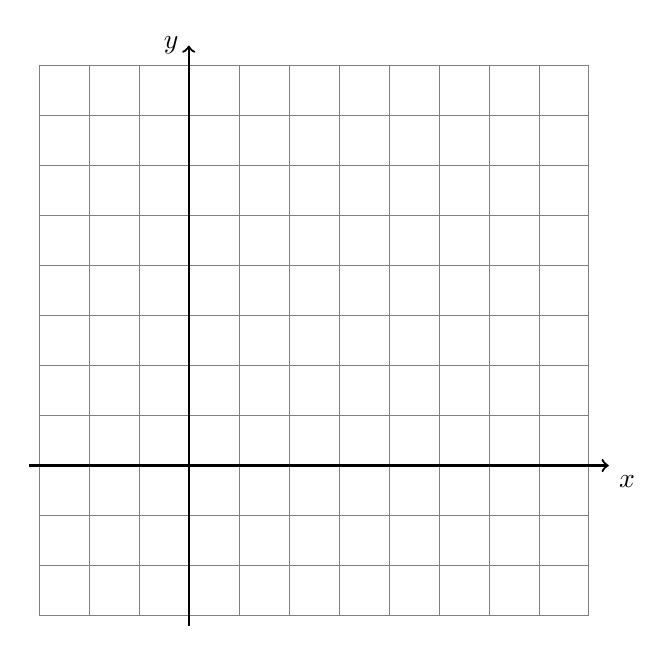
\begin{tikzpicture}[scale=.635]
  \draw [help lines] (-3,-3) grid (8,8);
  \draw [thick, ->] (-3.2,0) -- (8.4,0) node [below right] {$x$};
  \draw [thick, ->] (0,-3.2)--(0,8.4) node [left] {$y$};
\end{tikzpicture}

\newpage
\item Three of the vertices of the parallelogram $ABCD$ are given: $A(-1, 1)$, $B(4,-1)$, $C(6, 6)$. Determine and state the coordinates of the fourth vertex, $D$, and mark and label it on the grid below. Draw the sides of the parallelogram.
  \begin{center}
    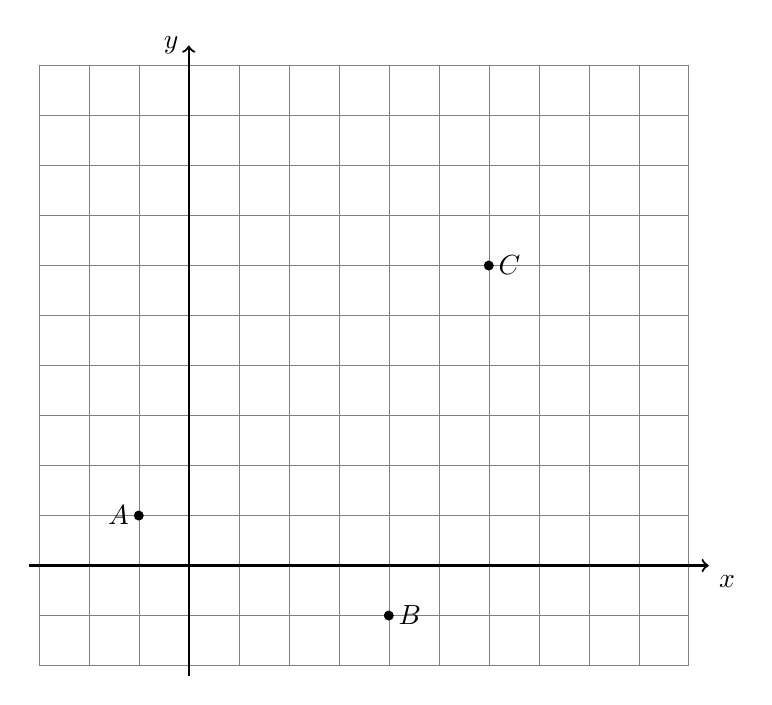
\begin{tikzpicture}[scale=.635]
      \draw [help lines] (-3,-2) grid (10,10);
      \draw [thick, ->] (-3.2,0) -- (10.4,0) node [below right] {$x$};
      \draw [thick, ->] (0,-2.2)--(0,10.4) node [left] {$y$};
      \fill (-1,1) circle[radius=0.1cm] node[left]{$A$};
      \fill (4,-1) circle[radius=0.1cm] node[right]{$B$};
      \fill (6,6) circle[radius=0.1cm] node[right]{$C$};
    \end{tikzpicture}
  \end{center}

  \item The parallelogram $BECA$ with vertices $B(-2,-1)$, $E(6,1)$, $C(4,7)$, and $A(-4,5)$ is shown. Use the midpoint formula to show that the diagonals $\overline{BC}$ and $\overline{EA}$ bisect each other. State that $M_{\overline{BC}} = M_{\overline{EA}}$ and the concluding statement.  Draw the diagonals and label the midpoint.\\[0.5cm]
      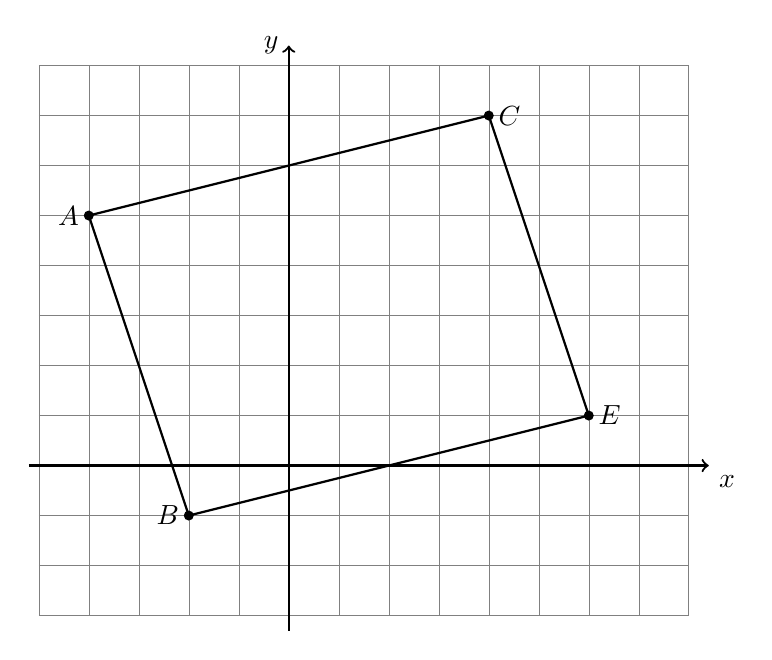
\begin{tikzpicture}[scale=.635]
        \draw [help lines] (-5,-3) grid (8,8);
        \draw [thick, ->] (-5.2,0) -- (8.4,0) node [below right] {$x$};
        \draw [thick, ->] (0,-3.3)--(0,8.4) node [left] {$y$};
        \draw [thick] (-2,-1)--(6,1)--(4,7)--(-4,5)--cycle;
        \fill (-2,-1) circle[radius=0.1cm] node[left]{$B$};
        \fill (6,1) circle[radius=0.1cm] node[right]{$E$};
        \fill (4,7) circle[radius=0.1cm] node[right]{$C$};
        \fill (-4,5) circle[radius=0.1cm] node[left]{$A$};
      \end{tikzpicture}

\end{enumerate}

\end{document}
